\documentclass[14pt, a4paper,reqno]{article}
\usepackage{hyperref}
\usepackage[warn]{mathtext}
\usepackage[utf8]{inputenc}
\usepackage[T2A]{fontenc}
\usepackage[russian]{babel}
\usepackage{amssymb, amsmath, multicol}
\usepackage{graphicx}
\usepackage[shortcuts,cyremdash]{extdash}
\usepackage{wrapfig}
\usepackage{gensymb}
\usepackage{floatflt}
\usepackage{lipsum}
\usepackage{verbatim}
\usepackage{concmath}
\usepackage{euler}
\usepackage{xcolor}
\usepackage{etoolbox}
\usepackage{fancyhdr}
\usepackage{subfiles}
\usepackage{enumitem}
\usepackage{amsthm}
\usepackage{indentfirst}
\usepackage{import}
\usepackage{multirow}
\usepackage{hhline}
\usepackage{calrsfs}

\DeclareMathOperator{\sign}{sign}

\RequirePackage[ left     = 1cm,
                 right    = 1cm,
                 top      = 2.0cm,
                 bottom   = 1.25cm,
                 includefoot,
                 footskip = 1.25cm ]{geometry}
                 
\setlength{\parskip}{ .5em plus .15em minus .08em }
\renewcommand {\baselinestretch}{ 1.07 }

\fancyhf{} % clear existing header/footer entries

\renewcommand{\footrulewidth}{ .0em }
\fancyfoot[C]{\texttt{\textemdash~\thepage~\textemdash}}

\makeatletter
\patchcmd\l@section{%
  \nobreak\hfil\nobreak
}{%
  \nobreak
  \leaders\hbox{%
    $\m@th \mkern \@dotsep mu\hbox{.}\mkern \@dotsep mu$%
  }%
  \hfill
  \nobreak
}{}{\errmessage{\noexpand\l@section could not be patched}}
\makeatother
\parindent = 1cm % отступ при красной строке⏎
\pagestyle{fancy}    
\renewcommand\qedsymbol{$\blacksquare$}

\newcommand{\when}[2]{
  \left. #1 \right|_{#2} \hspace
}
\renewcommand{\kappa}{\varkappa}
\RequirePackage{caption2}
\renewcommand\captionlabeldelim{}
\newcommand*{\hm}[1]{#1\nobreak\discretionary{}

\DeclareSymbolFont{T2Aletters}{T2A}{cmr}{m}{it}
{\hbox{$\mathsurround=0pt #1$}}{}}
% Цвета для гиперссылок
\definecolor{linkcolor}{HTML}{000000} % цвет ссылок
\definecolor{urlcolor}{HTML}{799B03} % цвет гиперссылок
 
\hypersetup{pdfstartview=FitH,  linkcolor=linkcolor,urlcolor=urlcolor, colorlinks=true}

\begin{document}

% НАЧАЛО ТИТУЛЬНОГО ЛИСТА
\begin{center}
  {\small ФЕДЕРАЛЬНОЕ ГОСУДАРСТВЕННОЕ АВТОНОМНОЕ ОБРАЗОВАТЕЛЬНОЕ\\ УЧРЕЖДЕНИЕ ВЫСШЕГО ОБРАЗОВАНИЯ\\ МОСКОВСКИЙ ФИЗИКО-ТЕХНИЧЕСКИЙ ИНСТИТУТ\\ (НАЦИОНАЛЬНЫЙ ИССЛЕДОВАТЕЛЬСКИЙ УНИВЕРСИТЕТ)\\ ФИЗТЕХ-ШКОЛА РАДИОТЕХНИКИ И КОМПЬЮТЕРНЫХ ТЕХНОЛОГИЙ}\\
  \hfill \break
  \hfill \break
  \hfill \break
  \Huge{Работа 3.4.4. \\ Петля гистерезиса (статический метод)}\\
\end{center}

\hfill \break
\hfill \break
\hfill \break
\hfill \break
\hfill \break
\hfill \break
\hfill \break
\hfill \break

\begin{flushright}
  \normalsize{Работу выполнил:}\\
  \normalsize{\textbf{Долгов Александр Алексеевич, группа Б01-106}}\\
\end{flushright}

\vspace*{\fill} %

\begin{center}
  \normalsize{\textbf{Долгопрудный, 2022}}
\end{center}

\thispagestyle{empty} % выключаем отображение номера для этой страницы

% КОНЕЦ ТИТУЛЬНОГО ЛИСТА

\newpage
\thispagestyle{plain}
\tableofcontents
\thispagestyle{plain}
\newpage
\section{Аннотация}

    В данной работе начальная кривая намагничивания ферромагнетиков и предельная петля гистерезиса исследовались
    статическим методом.

\section{Теоретические сведения}

    Если состояние некоторой системы зависит не только от мгновенных значений внешних параметров, 
    но и от истории их изменения, то говорят, что в системе имеет место \textbf{гистерезис}. Примером
    является зависимость намагниченности $M$ от напряжённсти магнитного поля $H$ в ферромагнетиках.
    
    На практике магнитные свойства ферромагнетиков изучают путём измерения не зависимости $M(H)$, а зависимости
    $B(H)$. Исследование образца обычно начинается в полностью размагниченном состоянии $(H = 0, B = 0)$. При
    увеличении поля $H$ индукция магнитного поля изменяется согласно соотношению:
    \begin{equation}\label{B-field}
        B(H) = \mu_0(H + M(H))
    \end{equation}
    Множество точек, удовлетворяющих уравнению \eqref{B-field}, называется \textbf{кривой намагничивания}. 
    Если кривая начинается в точки $(H = 0, B = 0)$ - \textbf{начальной кривой намагничивания}. Наклон кривой 
    характеризуется дифференциальной магнитной приницаемостью 
    \begin{equation*}
        \mu_{дифф} = \frac{1}{\mu_0}\frac{B}{H}
    \end{equation*}

    \begin{wrapfigure}{r}{0.4\textwidth}
        \begin{center}
            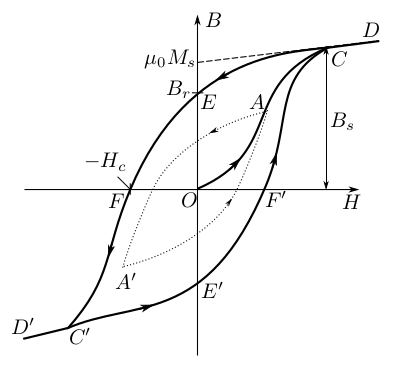
\includegraphics[width = 0.4\textwidth]{images/picture_1.png}
        \end{center}
    \caption{Характерный вид петли гистерезиса}
    \end{wrapfigure}

    Рассмотрим процесс гистерезиса в ферромагнетиках более детально. Пусть начальное состояние образца задаётся условиями
    $(H = 0, B = 0)$. Будем увеличивать поле $H$ до тех пор, пока поле $M$ меняется. Это перестанет происходить, при достижении
    некоторого поля $H_s$. Пусть полю $H_s$ соответствует поле $B_s$, которое назовём \textit{индукцией насыщения}. Точку
    $(H_s, B_s)$ на координатной плоскости назовём точкой $C$. Достигнув точки $C$, будем уменьшать поле $H$. Вследствие
    взаимодействия доменов друг с другом путь пойдёт не по начальной кривой, а выше неё.
    
    При $H = 0$ в образце сохраняется собственная намагниченность. Соответствующее значение индукции магнитного поля $B_r$
    называют \textit{остаточной индукцией}. Значение $B = 0$ достигается лишь при $H = -H_c$, где величина $H_c > 0$ называется
    \textit{коэрцитивным полем} (\textit{коэрцитивной силой}). При дальнейшем умешьшении поля $H$ до $-H_s$, образец выходит
    на насыщение в противоположную сторону. Если в точке $C$ насыщение не было достигнуто, то аналогичным образом получится 
    цикл меньшей площади. Если в точке $C$ насыщение всё же было достигнуто, то полученный цикл называется \textbf{предельной
    петлёй гистерезиса}.

    Характерный вид петли гистерезиса изображён на рисунке 1.

\section{Методика измерений}

    \begin{figure}[h]
        \begin{center}
            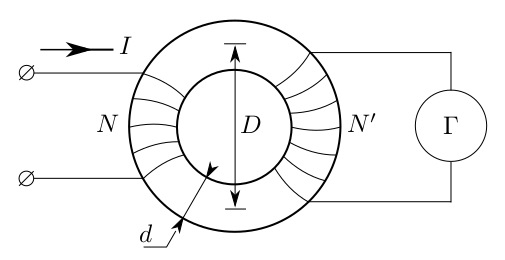
\includegraphics[width = 0.6\textwidth]{images/picture_2.png}
        \end{center}
    \caption{Характерный вид петли гистерезиса}
    \end{figure}
    На тороидальный сердечник, изготовленынй из исследуемого образца, равномерно намотана намагничивающая обмотка с числом витков
    $N$, а поверх неё - измерительная обмотка с числом виков $N'$ (см. рис. 2). При скачкообразном изменении тока в намагничивающей
    обмотке в измерительно обмотке возникает ЭДС индукции. Ток, вызванный этой ЭДС, регистрируется гальванометром Г, работающим в
    баллистическом (импульсном) режиме, то есть его отклонение пропорционально полному заряду $\Delta q$, протёкшему через него.
    
    Поле $H$ в сердечнике пропорционально току $I$ в намагничивающей обмотке, а изменение магнитной индукции - заряду $\Delta q$.
    Таким образом, изменяя токи $I$ и суммируя отклонения $\Delta q$ гальванометра Г, можно получить зависимость $B(H)$ для материала
    сердечника.

    Поле $H$ для тороидальной катушки можно найти по формуле:
    \begin{equation}\label{H-field}
        H = \frac{IN_0}{2\pi R},
    \end{equation}
    где $N_0$ - число витков, $R$ - расстояние от оси тора. Пусть в намагничивающей катушке ток скачкообразно изменился на величину
    $\Delta I$. Тогда поле в тороиде изменится пропорционально: $\Delta H \propto \Delta I$. Изменение поля $H$ в свою очередь приводит
    к изменению магнитного потока $\Phi$ в сердечнике, и в измерительной обмотке сечения $S$ с числом витков $N'$ возникает ЭДС
    индукции:
    \begin{equation*}
        \mathcal{E} = -\frac{d\Phi}{dt} = -SN'\frac{dB}{dt}
    \end{equation*}
    Поскольку гальванометр работает в баллистическом режиме, то при протекании импульса тока первый отброс \glqqзайчика\grqq
    пропорционален величине прошедшего через гальванометр заряда:
    \begin{equation*}
        \Delta x = \frac{\Delta q}{b},
    \end{equation*}
    где $b$ - константа, называемая \textit{баллистической постоянной гальванометра}. Свяжем $\Delta x$ и $\Delta B$:
    \begin{equation}\label{delta_x}
        |\Delta x| = \frac{1}{b}\left|\int I dt\right| = \frac{1}{bR}\left|\int \mathcal{E}dt\right| = 
        \frac{SN'}{bR}\left|\int dB\right| = \frac{SN'}{bR}|\Delta B|,
    \end{equation}
    где $R$ - сопротивление измерительного тороида.

    \begin{wrapfigure}{l}{0.2\textwidth}
        \begin{center}
            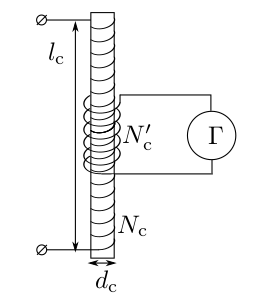
\includegraphics[width = 0.2\textwidth]{images/picture_3.png}
        \end{center}
    \caption{Cхема для калиброки гальванометра}
    \end{wrapfigure}
    Баллистическую постоянную можно определить, если провести аналогичные измерения, взяв вместо тороида с сердечником пустотелый
    соленоид с числом витков $N_c$, на который намотана короткая измерительная катушка с числом витков $N'_c$ (см. рис. 3). Магнитная
    индукция в пустом соленоиде находится по формуле:
    \begin{equation}\label{B_in_solenoid}
        B_c = \mu_0 H_c \approx \frac{N_c}{l_c}I_c, 
    \end{equation}
    где $l_c$ - длина пустотелого соленоида, $I_c$ - сила текущего через него тока. Показания гальванометра при изменении тока в соленоиде 
    находятся по формуле, аналогичной
    \eqref{delta_x}:
    \begin{equation*}
        |\Delta x_c| = \frac{S_сN'_c}{bR_c}|\Delta B_c|,
    \end{equation*}
    С учётом \eqref{B_in_solenoid} имеем:
    \begin{equation}\label{delta_x_c}
        |\Delta x_c| = \frac{S_сN'_c N_c}{bR_c l_c}|\Delta I_с|,
    \end{equation}
    \\
    \\
    \noindentгде $R_c$ - полное сопротивление измерительной цепи соленоида, $S_c$ - площадь поперечного сечения соленоида. Разделив
    \eqref{delta_x} на \eqref{delta_x_c}, получим формулу, не содержающую баллистической постоянной:
    \begin{equation}\label{delta_B}
        \boxed{|\Delta B| = \mu_0 \frac{N'_c}{N'}\frac{R}{R_c}\frac{S_c}{S}\frac{N_c}{l_c}\frac{|\Delta I_с|}{|\Delta x_c|}|\Delta x|}
    \end{equation}

\section{Экспериментальная установка}

    Схема экспериментальной установки представлена на рисунке 4. Генератор токов намагничивания (ГТН) позволяет
    скачками менять токи в намагничивающей обмотке тороида. Одинаковые скачки $\Delta I$ вызывают разные отклонения
    зайчика гальванометра $\Delta x$ на разных участках петли. Поэтому генератор меняет ток неравномерно: большими
    скачками выблизи насыщения и малыми вблизи нуля.

    Ток в намагничивающей обмотке измеряется цифровым мультиметром А. Переключатель $П_1$ позволяет менять направление
    тока в первичной обмотке. Чувствительность гальванометра Г во вторичной обмотке цепи можно менять с помощью магазина
    сопротивлений $R_M$. Ключ $K_1$ предохраняет гальванометр от перегрузок и замыкается только на время измерений отклонения
    зайчика. Ключ $K_0$ служит для мгновенной остановки зайчика. Переключателем $П_2$ можно изменять направление тока
    через гальванометр.

    Схема на рисунке 5 отличается от схемы на рисунке 4 только тем, что вместо тороида в ней подключён калибровочный соленоид.

    \begin{figure}[h]
        \begin{center}
            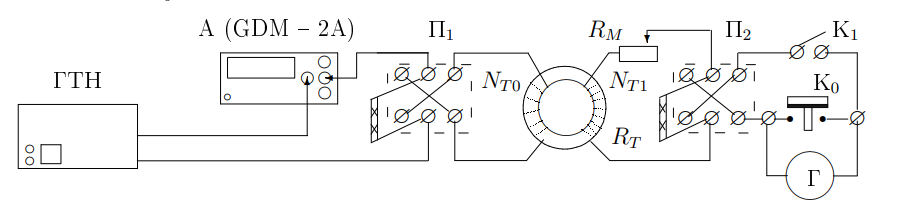
\includegraphics[width = 0.6\textwidth]{images/picture_4.png}
        \end{center}
    \caption{Схема установки для исследования петли гистерезиса}
    \end{figure}

    \begin{figure}[h]
        \begin{center}
            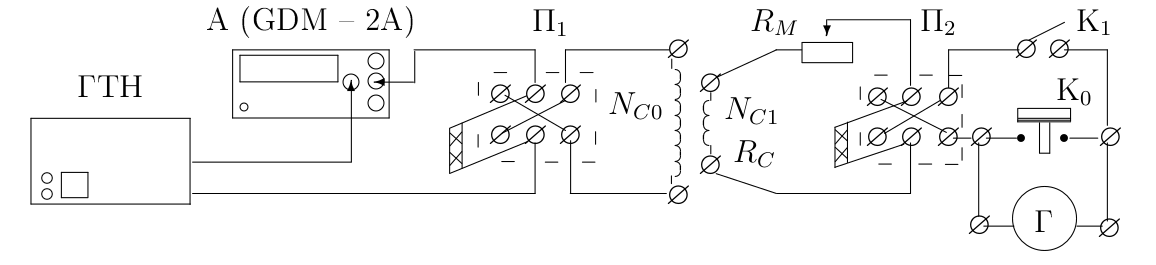
\includegraphics[width = 0.6\textwidth]{images/picture_5.png}
        \end{center}
    \caption{Схема установки для калибровочного гальванометра}
    \end{figure}

\section{Оборудование и экспериментальные погрешности}

    \subsection{Параметры установки}

        \textbf{Количество витков в намагничивающей обмотке тороида:} N = 1750

        \textbf{Количество витков в измерительной обмотке тороида:} N' = 300

        \textbf{Количество витков в намагничивающей катушке:} $N_c$ = 940
        
        \textbf{Количество витков в измерительной катушке:} $N'_c$ = 500

        \textbf{Диаметр тороида:} $d$ = 1 см

        \textbf{Диаметр соленоида:} $d_c$ = 7 см

        \textbf{Средний диаметр тороида (среднее расстояние до его оси):} $D$ = 10 см

        \textbf{Длина соленоида:} $l_c$ = 80 см

        \textbf{Сопротивление цепи тороида:} $R$ = 5.6 Ом

        \textbf{Сопротивление цепи соленоида:} $R_c$ = 46 Ом

    \subsection{Погрешности измеряемых величин}

    Из формулы \eqref{H-field} получаем выражение для погрешности напряжённости магнитного поля:
    \begin{equation*}
        \sigma_H =  \frac{N}{\pi D}\sigma_I,
    \end{equation*}

    В ходе работы сила тока измерялась с абсолютной погрешностью $\sigma_I = 10^{-4} A$. Следовательно:
    \begin{equation*}
        \sigma_H = 0.6 \frac{А}{м}
    \end{equation*}

    Величина $\Delta x$ измерялась с абсолютной погрешностью $\sigma_x = 0.5\ мм$.

    Запишем формулу \eqref{delta_B} в более компактном виде:
    \begin{equation*}
        |\Delta B| = k|\Delta x|,\ k = \mu_0 \frac{N'_c}{N'}\frac{R}{R_c}\frac{d_c^2}{d^2}\frac{N_c}{l_c}\frac{|\Delta I_c|}{|\Delta x_c|}
    \end{equation*}

    Таким образом, погрешность $\sigma_k$ коэффициента $k$ вычисляется по формуле:
    \begin{equation*}
        \sigma_k = k \sqrt{\left(\frac{\sigma_I}{\Delta I}\right)^2 + \left(\frac{\sigma_x}{\Delta x_c}\right)^2}
    \end{equation*}

    Соответственно, погрешность $\sigma_B$ величины $|\Delta B|$ вычисляется по формуле:
    \begin{equation*}
        \sigma_B = |\Delta B|\sqrt{\left(\frac{\sigma_k}{k}\right)^2 + \left(\frac{\sigma_x}{\Delta x}\right)^2}
    \end{equation*}

\section{Измерения и обработка их результатов}

    \subsection{Калибровка гальванометра}

        Для калибровки гальванометра была проведено одно измерение $|\Delta x_c|(I)$. Результаты следующие:
        \begin{equation*}
            |\Delta I_c| = 1.301\ A
        \end{equation*}
        \begin{equation*}
            |\Delta x| = 49\ мм
        \end{equation*}
        Таким образом:
        \begin{equation*}
            k = (3.20\pm 0.03)\ \frac{Тл}{м}
        \end{equation*}

    \subsection{Наблюдение предельной петли гистерезиса}

        По описанной выше схеме была измерена зависимость $\Delta I(\Delta x)$, по которой восстановлена зависимость
        $B(H)$. Результаты измерений и промежуточных расчётов представлены в таблице 1. По этим данным также построен
        график 1.

\section{Вывод}

        Вид предельной петли гистерезиса совпадает с ожидаемым. Тем не менее, начальная кривая намагничивания происходит
        выше, чем должна по предсказаниям теории. Это возможно объяснить тем, что в ходе исследования начальной кривой
        образец не был должным образом размагничен, и следовательно в нём присутствовало ненулевое поле $M$.

\newpage
\section{Приложения}

    \subsection{Таблицы}
    \begin{center}
        \captionof{table}{Исследование предельной петли гистерезиса}
        \begin{tabular}{|c|c|c|c|c|}
            \hline
            I, А     & $\Delta x$, мм & H, А/м   & $\Delta B$, мТл & $\sigma_B$, мТл    \\ \hline\hline
            1.7294   & 71             & 963.3	& -227            & 3  \\ \hline
            0.941    & 53             & 524.2	& -170            & 2  \\ \hline
            0.5844   & 14             & 325.5	& -45             & 2  \\ \hline
            0.4873   & 11             & 271.4	& -35             & 2  \\ \hline
            0.3977   & 9              & 221.5	& -29             & 2  \\ \hline
            0.3549   & 5              & 197.7	& -16             & 2  \\ \hline
            0.3241   & 7              & 180.5	& -22             & 2  \\ \hline
            0.2836   & 5              & 158.0	& -16             & 2  \\ \hline
            0.2459   & 7              & 137.0	& -22             & 2  \\ \hline
            0.1862   & 8              & 104.0	& -27             & 2  \\ \hline
            0.1098   & 15             & 61.2	& -48             & 2  \\ \hline
            0        & 45             & 0	    & -144            & 2  \\ \hline
            -0.1097  & 55             & -61.1	& -176            & 2  \\ \hline
            -0.186   & 82             & -103.6	& -263            & 3  \\ \hline
            -0.2466  & 77             & -137.4	& -247            & 3  \\ \hline
            -0.2847  & 87             & -158.6	& -279            & 3  \\ \hline
            -0.3238  & 54             & -180.4	& -173            & 2  \\ \hline
            -0.3545  & 60             & -197.5	& -192            & 3  \\ \hline
            -0.3977  & 80             & -221.5	& -256            & 3  \\ \hline
            -0.4853  & 48             & -270.3	& -154            & 2  \\ \hline
            -0.584   & 88             & -325.3	& -282            & 3  \\ \hline
            -0.9412  & 81             & -524.3	& -259            & 3  \\ \hline
            -1.7296  & -65            & -963.5	& 208             & 3  \\ \hline
            -0.9425  & -43            & -525.0	& 138             & 2  \\ \hline
            -0.5846  & -21            & -325.6	& 67              & 2  \\ \hline
            -0.4873  & -11            & -271.4	& 35              & 2  \\ \hline
            -0.3981  & -5             & -221.8	& 16              & 2  \\ \hline
            -0.3551  & -4             & -197.8	& 13              & 2  \\ \hline
            -0.3242  & -5             & -180.6	& 16              & 2  \\ \hline
            -0.2856  & -7             & -159.1	& 22              & 2  \\ \hline
            -0.2468  & -7             & -137.5	& 22              & 2  \\ \hline
            -0.1862  & -10            & -103.7	& 32              & 2  \\ \hline
            -0.1098  & -14            & -61.2	& 45              & 2  \\ \hline
            0        & -45            & 0	    & 144             & 2  \\ \hline
            0.1097   & -55            & 61.1	& 176             & 2  \\ \hline
            0.1861   & -81            & 103.7	& 259             & 3  \\ \hline
            0.2482   & -73            & 138.3	& 234             & 3  \\ \hline
            0.2842   & -91            & 158.3	& 291             & 3  \\ \hline
            0.324    & -59            & 180.5	& 189             & 3  \\ \hline
            0.3547   & -65            & 197.6	& 208             & 3  \\ \hline
            0.3978   & -85            & 221.6	& 272             & 3  \\ \hline
            0.4854   & -52            & 270.4	& 166             & 2  \\ \hline
            0.5841   & -98            & 325.4	& 314             & 4  \\ \hline
            0.942    & -87            & 524.7	& 27              & 3  \\ \hline
            1.723    &                & 959.8	& 0               &    \\ \hline
        \end{tabular}
    \end{center}

    \newpage
    \begin{center}
        \captionof{table}{Исследование начальной кривой намагничивания}
        \begin{tabular}{|c|c|c|c|c|}
            \hline
            I, А    & $\Delta x$, мм & H, А/м   & $\Delta B$, мТл & $\sigma_B$, мТл \\ \hline\hline
            0       & -47            &  0       &  150.5          &  3.4    \\ \hline
            0.1098  & -39            &  61.2    &  124.9          &  2.8    \\ \hline
            0.1861  & -62            &  103.7   &  198.5          &  0.6    \\ \hline
            0.2476  & -47            &  137.9   &  150.5          &  0.5    \\ \hline
            0.2848  & -55            &  158.6   &  176.1          &  0.4    \\ \hline
            0.3239  & -33            &  180.4   &  105.7          &  0.3    \\ \hline
            0.3547  & -38            &  197.6   &  121.7          &  0.4    \\ \hline
            0.3977  & -63            &  221.5   &  201.7          &  0.2    \\ \hline
            0.4853  & -48            &  270.3   &  153.7          &  0.3    \\ \hline
            0.584   & -10            &  325.3   &  326.6          &  0.3    \\ \hline
            0.9431  & -93            &  525.3   &  297.8          &  0.6    \\ \hline
            1.7303  &                &  963.9   &  0              &         \\ \hline
        \end{tabular}
    \end{center}

    \newpage
    \subsection{Графики}

    \textbf{График 1. Предельная петля гистерезиса и начальная кривая намагничивания}
    \begin{center}
        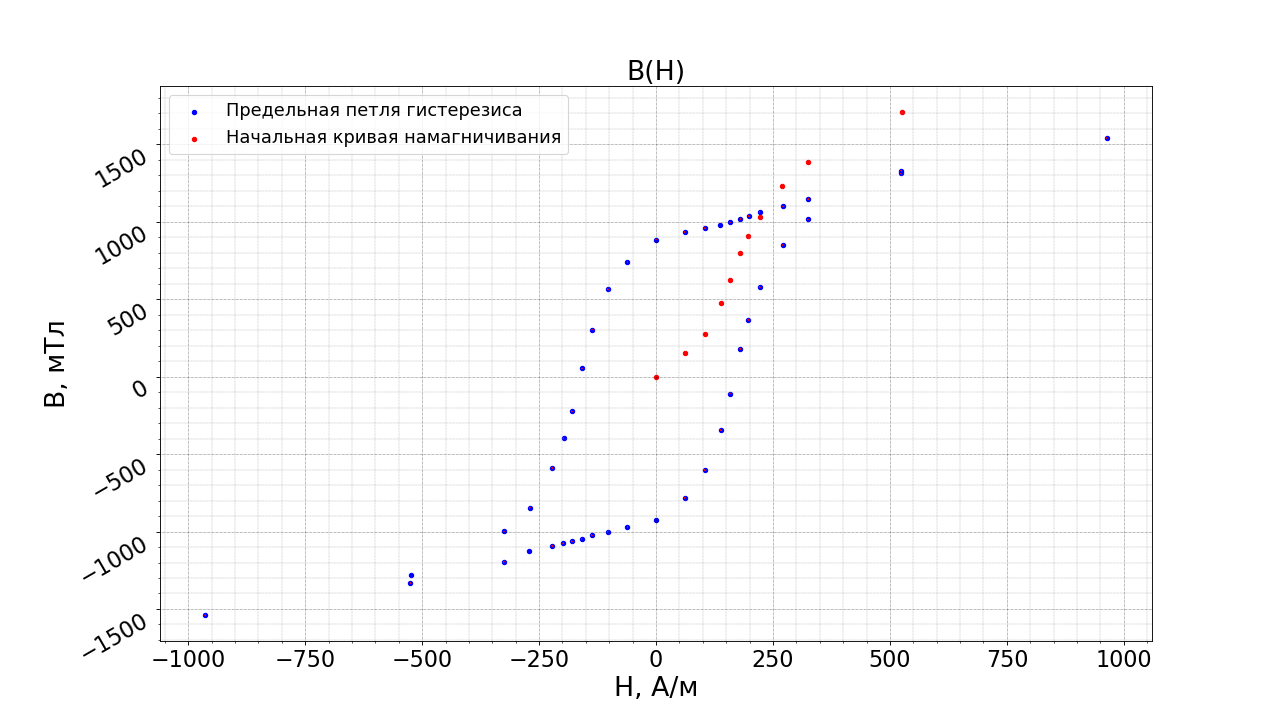
\includegraphics[width = \textwidth]{images/graph.png}
    \end{center}

\end{document}
